\documentclass[11pt]{article}

% Standalone academic manuscript.
\usepackage[margin=1in]{geometry}
\usepackage{lmodern}
\usepackage{amsmath,amssymb}
\usepackage{float}
\usepackage{algpseudocode}
\usepackage{booktabs}
\usepackage{graphicx}
\usepackage{array}
\usepackage{tikz}
\usetikzlibrary{arrows.meta,calc}
\usepackage{hyperref}
\hypersetup{colorlinks=true,linkcolor=blue,citecolor=blue,urlcolor=blue}
\emergencystretch=2em

\newcommand{\care}{\textsc{CARE}}
\newcommand{\botans}{\bot}
\newcommand{\gold}{\mathcal{G}}
\newcommand{\sources}{\mathcal{S}}
\newfloat{algorithm}{tbhp}{loa}
\floatname{algorithm}{Algorithm}

\title{\care: Conditional Answer Repair with Source-Anchored Evidence\\
for Long-Horizon Conversational Memory}
\author{Anonymous authors}
\date{}

\begin{document}
\maketitle

\begin{abstract}
Long-horizon conversational question answering depends on finding the right
past turn and preserving its speaker and temporal scope under a limited
context budget. We study this answer-time problem and introduce \care{}
(Conditional Answer Repair with Source-Anchored Evidence), a bounded reader
over immutable, addressable conversation turns. A first pass answers from a
sparse-retrieval bundle while reporting cited source IDs and searches for
missing evidence. A source-binding gate can trigger one expanded retrieval
and reading pass. On all 1,986 questions in ten LoCoMo conversations, using
Qwen3-8B with an 8K context window, \care{} scores 0.5256. With the same
reader, first-bundle size, and repair policy, dense initial retrieval scores
0.4994 (paired difference 0.0261). Selecting \care{}'s saved second-pass
outputs raises its score by 0.0667 but reverses 46 formerly correct
refusals; the corresponding dense-reader repair reverses 68. A separate
context-coverage audit shows that a fixed 8K history
loses every annotated answer source on 1,060 answerable questions; when all
annotated sources remain visible, the window-limited reader is stronger.
These results characterize both the benefit and the abstention risk of
conditional evidence repair. The larger gain over the earlier raw-turn dense
pipeline changes its prompt and evidence budget; the matched-reader result
is the more specific test of initial retrieval choice.
\end{abstract}

\section{Introduction}
\label{sec:introduction}

\subsection{The Answer-Time Evidence Bottleneck}

Long-running agents must answer questions about interactions distributed
across sessions. Their histories can exceed the model's working context,
while the decisive evidence may be a short remark made months earlier.
A bounded context therefore creates an \emph{access problem}: the answerer
may never see the relevant turn. Even when retrieval surfaces a related
turn, it can create a \emph{binding problem}: a first-person statement may
be attributed to the wrong speaker, or an update may be mistaken for an
older state. Temporal questions add a further requirement to relate an
expression such as ``last year'' to the date of the session in which it
appeared. LoCoMo makes these problems concrete through long, multi-session
dialogues and questions spanning factual, temporal, inferential, contextual,
and unsupported-premise cases~\cite{maharana2024locomo}.

Long-term memory research has rightly examined extraction, consolidation,
linking, and learned write decisions. These mechanisms govern what survives
in a persistent store. Nevertheless, a store can contain the answer while
the reader fails to select or interpret it. Conversely, a compressed note
can discard the identity or date needed to check a later answer. We therefore
separate memory \emph{construction} from memory \emph{use} and ask: given
immutable, addressable source turns, how should a bounded answerer select,
verify, and if needed repair the evidence it reads?

\subsection{From Retrieval to Conditional Evidence Repair}

A fixed top-$k$ retrieval system makes one selection before generation. This
is attractive for cost, but a lexically or semantically plausible hit need
not answer the question, and the reader has no formal way to communicate
which evidence remains missing. \care{} makes this interaction explicit.
Its first pass ranks original turns sparsely and asks the answer model for
three outputs: a short answer, supporting source IDs, and at most two
targeted searches. A deterministic gate checks whether the claimed support
is among the visible turns and whether selected speaker and event constraints
hold. Only invalid or evidence-poor responses initiate a broader retrieval
pass. The second pass adds stemmed lexical matches, local session neighbors,
and search results requested by the reader. Both passes retain the original
turn text and its metadata.

This design contributes an operational distinction between \emph{retrieval
coverage} and \emph{answer grounding}. The first is whether a relevant
source was shown; the second is whether the proposed answer names an
admissible visible source and respects the available binding checks. A
source identifier is an auditable handle, not a machine-verifiable proof of
semantic entailment. The gate is intentionally narrow, but it provides a
bounded opportunity to correct several observable failures without a
second call on every question.

\subsection{Contributions and Scope}

\begin{enumerate}
  \item \textbf{A source-anchored read interface.} We formulate an answer-time
  memory procedure over immutable, dated, speaker-attributed turns. The
  reader's structured response exposes both claimed support and missing
  evidence, and a deterministic gate controls one repair pass.
  \item \textbf{A complete comparison and matched-reader ablation.} We evaluate
  \care{} and three context-access controls on the same 1,986 LoCoMo
  questions with a pinned Qwen3-8B model. A further four-arm comparison
  holds the reader prompt and top-eight evidence size fixed while varying
  initial retrieval and conditional repair, reporting task score, source
  recall, inference calls, and server-measured tokens.
  \item \textbf{A diagnosis of repair and context coverage.} We score the
  saved first read against its final answer and audit which annotated source
  turns survived an 8K fixed context. Together these analyses expose a gain
  on answerable questions, a loss on unsupported questions, and the coverage
  regime in which direct context reading is stronger.
\end{enumerate}

The central empirical claim is that sparse selection and conditional repair
improve a same-reader dense control under the studied 8K budget, with a
measurable refusal cost from repair. The experiments do not establish an
advantage over an untruncated context or demonstrate that a learned memory
writer caused the gain.

\section{Related Work}
\label{sec:related}

\subsection{Persistent Memory and Write-Time Organization}

MemGPT manages a finite working context by moving information through a
hierarchy of in-context and external storage~\cite{packer2023memgpt}.
Mem0 examines extraction, consolidation, and retrieval of long-term
memories, including a graph-enhanced variant~\cite{chhikara2025mem0}.
A-Mem organizes atomic notes with dynamic links and revises their contextual
attributes~\cite{amem2025}, while Memory-R1 studies learned write operations
and an answering policy~\cite{memoryr12025}. These lines of work address
the structure and evolution of the stored memory. Our experiment holds the
source history fixed and investigates the downstream reading operation.
The two directions are compatible: a future writer could organize derived
memories while retaining original source IDs for answer-time verification.

\subsection{Adaptive Retrieval and Corrective Reading}

Retrieval-augmented generation selects external text to condition a generator
~\cite{lewis2020rag}. FLARE retrieves again during generation when a
low-confidence continuation calls for more information~\cite{jiang2023active}.
Self-RAG learns when to retrieve and reflect on retrieved passages and generated
claims~\cite{asai2023selfrag}. Adaptive-RAG selects among no retrieval,
single-step, and iterative strategies based on question complexity
~\cite{jeong2024adaptive}. CRAG evaluates retrieved evidence and invokes
corrective retrieval actions when its quality is low~\cite{yan2024crag}.
Thus, conditional retrieval and corrective generation are established ideas.
\care{} studies a narrower operation: a frozen reader of speaker- and
date-attributed conversation turns reports a missing-evidence search and
cited source IDs; a rule-based source-binding gate allows at most one further
read. The present experiments do not demonstrate superiority to these
adaptive RAG methods under a shared implementation.

\subsection{Query-Time Conversational Memory}

MemR$^3$ explicitly tracks grounded evidence and unresolved gaps while
routing among retrieval, reflection, and answering actions for conversational
memory~\cite{du2026memr3}. CueMem uses extracted cues to reconstruct a
query-relevant context from the original source turns and their temporal and
semantic neighbors~\cite{wang2026cuemem}. LiveCtx retains original sessions
and selects or compresses context after observing the question
~\cite{liu2026livectx}. These studies show that neither explicit evidence
gaps nor return to original dialogue turns is, by itself, a novel mechanism.
Relative to them, \care{} combines immutable source handles, a structured
first-reader response, narrow attribution checks, and a two-call ceiling.
Whether this combination yields a better quality--cost frontier than those
systems remains an open empirical comparison: published scores use different
backbones, budgets, and evaluation rules.

\subsection{Long-Horizon Evaluation}

LoCoMo contains multi-session histories and questions about factual,
temporal, and contextual information, as well as unsupported premises
~\cite{maharana2024locomo}. We use reference answers and annotated source
IDs only after inference. LongMemEval tests complementary abilities such as
multi-session reasoning, temporal updates, and abstention across longer
histories~\cite{wu2024longmemeval}; it is a necessary external validation
target for this read path. BERTScore~\cite{zhang2020bertscore} measures
semantic similarity between a prediction and a reference; it provides a
complementary text metric but cannot establish whether the cited conversation
turn entails the prediction. Claim-level evidence analysis, as in
RAGChecker~\cite{ru2024ragchecker}, would test a stronger notion of grounding
than the present source-ID checks. This distinction motivates reporting
answer quality, source coverage, and refusal accuracy separately.

\section{Formal Problem Setting}
\label{sec:setting}

\subsection{Source-Addressable Conversation Memory}

Let a conversation be a sequence of original turns
\begin{equation}
\sources = (s_1,\ldots,s_N),\qquad
s_i=(\mathrm{id}_i,\mathrm{session}_i,t_i,p_i,x_i),
\label{eq:source}
\end{equation}
where $t_i$ is the session date, $p_i$ the speaker, and $x_i$ the turn text
with an available image caption appended as text. The source identifier
$\mathrm{id}_i$ is unique within a conversation. The corpus is immutable
during answering. For a question $q$, a method chooses a visible bundle
$B(q)\subseteq\sources$ whose serialized length does not exceed its
method-specific evidence budget $L$, then produces an answer $a$ or an
abstention $\botans$. Each
non-abstaining answer may additionally carry a citation set $C$ of source
IDs. We distinguish the \emph{candidate pool} examined by retrieval from
the \emph{visible bundle} actually serialized into the reader prompt; the
character budget can exclude candidates.

\subsection{Answer Quality, Coverage, and Cost}

Let $y_q$ be the benchmark reference answer and $m_q(a,y_q)$ the applicable
LoCoMo score. For a method $\pi$ that chooses bundles and calls a reader,
the empirical objective under a call budget is
\begin{equation}
\max_{\pi}\ \frac{1}{|\mathcal{Q}|}\sum_{q\in\mathcal{Q}}m_q(a_{\pi,q},y_q)
\quad\text{subject to}\quad |\mathrm{serialize}(B_{\pi,q})|\leq L,
\quad n_{\pi,q}\leq 2.
\label{eq:objective}
\end{equation}
This expression states the measured task objective; $y_q$ is never available
to $\pi$ at inference. For diagnostic analysis only, let $G_q$ denote the
dataset's annotated answer-source IDs. We measure source recall by the
fraction of $G_q$ in $B(q)$ and classify a fixed context by whether it
contains all, some, or none of $G_q$. Source recall is neither the task
score nor a guarantee of factual correctness: annotations can be incomplete,
and a reader can fail despite seeing every annotated turn.

For \care{}, $L$ is 10,000 serialized characters; the context baseline is
instead constrained by the model's 8,192-token window. All main methods draw
their context from the same original histories, but their selection and
answer prompts differ. The experiments therefore compare complete inference
pipelines, not isolated retrieval algorithms.

\section{The \care{} Framework}
\label{sec:method}

\subsection{Architecture Overview}

Figure~\ref{fig:care-architecture} presents the method as an answer-time
control loop over immutable conversation turns. The top path is the common
case: sparse retrieval supplies a compact source bundle to a reader that
returns both an answer and its proposed evidence. A source-binding gate accepts
an admissible response or an explicit abstention. When the first pass exposes
a missing-evidence search, fails a source-binding check, or abstains under a
risk cue, the lower path expands the evidence and invokes the reader once
more. This arrangement separates source storage, evidence selection,
answer generation, and source-binding checks. It also makes the repair budget an
explicit property of the architecture rather than an unrestricted agent loop.

\begin{figure}[t]
\centering
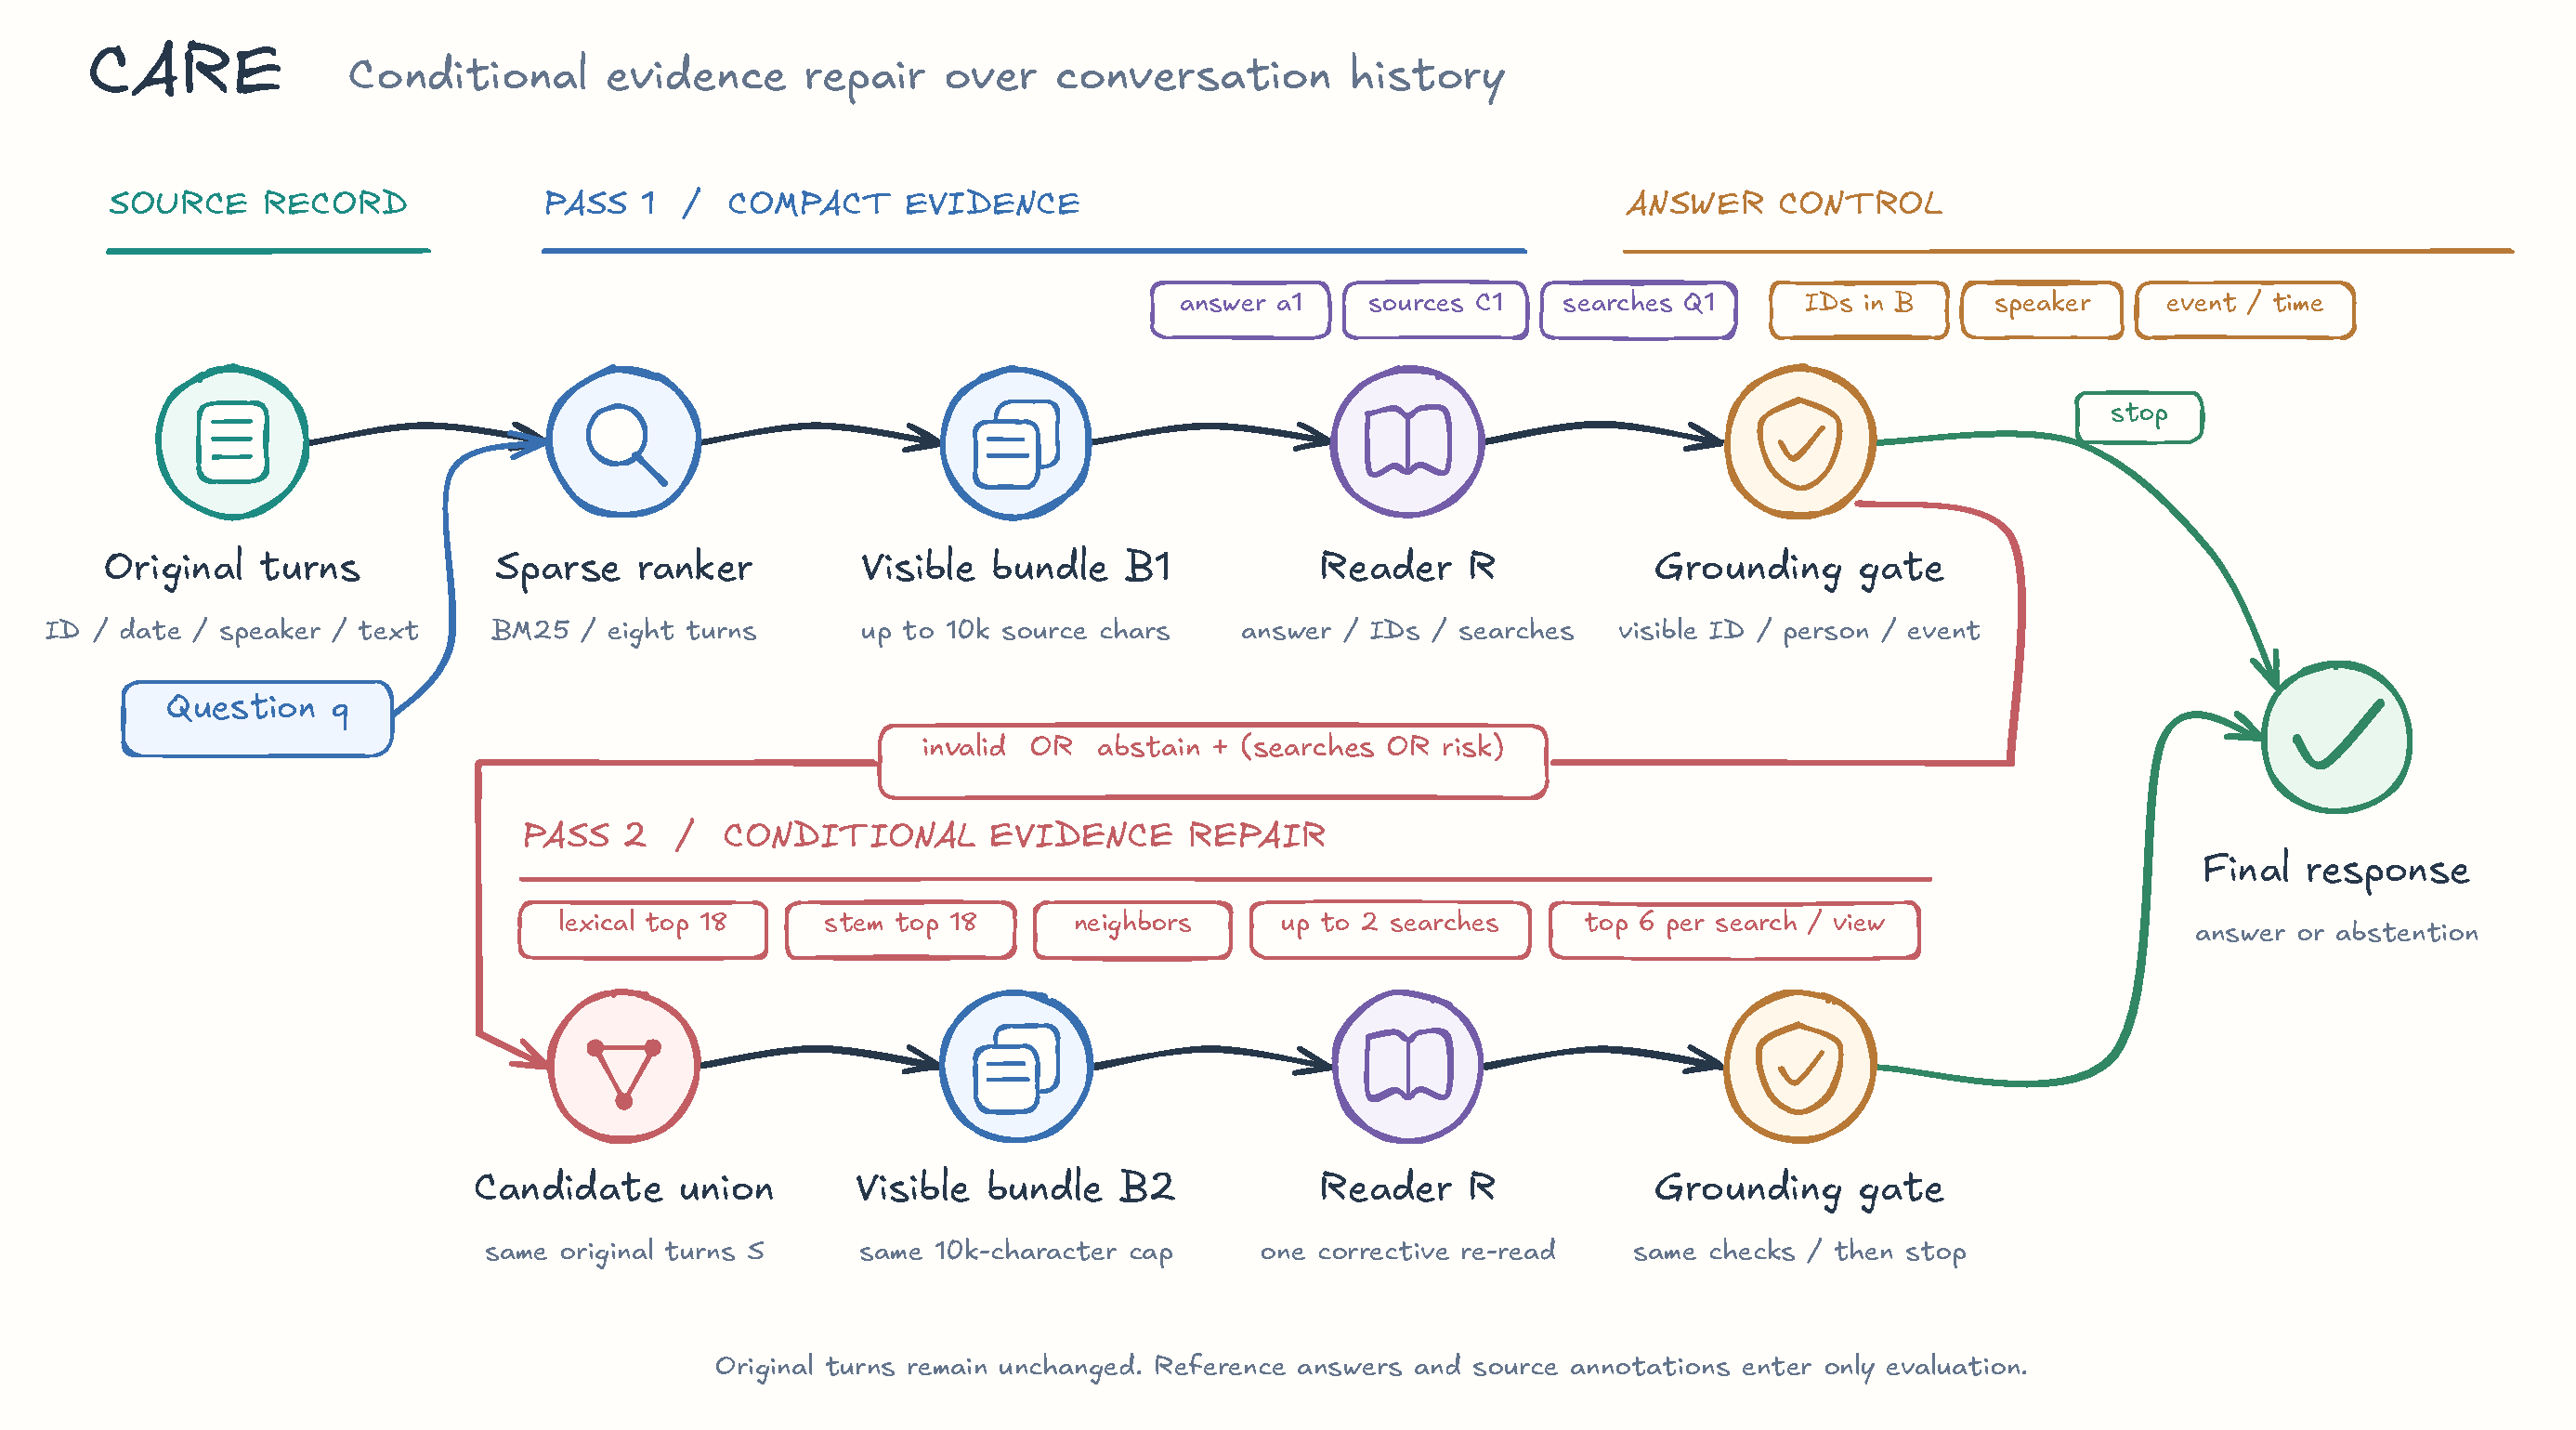
\includegraphics[width=\linewidth]{figures/care_architecture_excalidraw.pdf}
\caption{Architecture of \care{}. Original turns retain speaker, date, and
source identity. The upper path answers from a small retrieved bundle; a
failed source-binding check or evidence gap activates one bounded expansion and
re-read. Gold annotations enter only the evaluation, not the inference path.}
\label{fig:care-architecture}
\end{figure}

\subsection{Stage 1: Immutable Source Index and Sparse Selection}

\care{} represents a conversation as the original turn sequence in
Eq.~\eqref{eq:source}. Each turn remains addressable by a unique ID and
retains its speaker and session date. The ranking index uses stopword-filtered
tokens from the speaker label and turn text; dates and IDs are retained for
reading but do not enter the lexical score. For a query $q$, the first pass
ranks turns with BM25 using $k_1=1.5$ and $b=0.75$:
\begin{equation}
\mathrm{score}(q,s_i)=\sum_{w\in q\cap s_i}
\log\!\left(1+\frac{N-\mathrm{df}_w+0.5}{\mathrm{df}_w+0.5}\right)
\frac{2.5 f_{wi}}{f_{wi}+1.5(0.25+0.75\ell_i/\bar\ell)}.
\label{eq:bm25}
\end{equation}
Here $f_{wi}$ is the token frequency in turn $i$, $\ell_i$ its indexed
length, and $\bar\ell$ the mean turn length. Source order resolves score
ties. The top eight turns form the first candidate bundle. Before each
reader call, a serialization of visible turns is formed as
an identifier, session date, speaker, and original text under a
10,000-character evidence cap.
This representation preserves the attribution needed to interpret
first-person statements and explicit relative dates.

\subsection{Stage 2: Reader Contract and Evidence-Gap Signal}

Given a visible bundle $B$, the frozen reader returns a compact JSON object
\begin{equation}
(a,C,Q)=R_{\theta}(q,B),\qquad |Q|\leq 2,
\label{eq:reader}
\end{equation}
where $a$ is a short answer, $C$ contains proposed supporting source IDs,
and $Q$ contains targeted searches for missing evidence. The prompt asks
for an explicit abstention, ``No information available,'' when the
question's premise is unsupported; supported answers should leave $Q$
empty. This is a structured interface between retrieval and reading: the
reader can answer from the current bundle or indicate what further evidence
would make the question decidable.

For temporal questions, the interface may include deterministic hints that
resolve explicit relative expressions against a source turn's session date,
for example ``last year'' against a dated turn. Hints are tied to source IDs
and are generated only for recognized date phrases. They do not infer
unstated events or overwrite source text.

\subsection{Stage 3: Deterministic Source-Binding Checks}

The returned IDs are filtered to the IDs actually visible in $B$. A
non-abstaining answer requires at least one remaining citation. For a
question naming one conversation speaker, a cited first-person claim must
bind to that speaker according to speaker labels and a rule-based textual
heuristic. Additional checks reject a citation when the question names one
of five recognized holidays absent from that turn or asks when an activity stopped
without a cessation cue in the cited text. Invalid JSON, an empty answer,
or a failed citation or binding check turns that pass into abstention and
records a failure reason. These rules detect specific attribution and event
errors; they are not an entailment verifier. In particular, retaining a
visible citation does not prove that the cited words justify the answer.

\subsection{Stage 4: Risk-Gated Retrieval and Answer Repair}

Let $r_1$ indicate a parse or binding failure on the first pass, and let
$\rho(q,P_1)$ flag a question or initial candidate pool $P_1$ with temporal,
update, cross-speaker, or plural-aggregation cues. The second-pass decision
is
\begin{equation}
\tau(q)=\mathbf{1}\!\left[
r_1\ \lor\
\bigl(a_1=\botans\ \land\ (Q_1\neq\varnothing\ \lor\ \rho(q,P_1))\bigr)
\right].
\label{eq:gate}
\end{equation}
An ordinary supported first-pass answer therefore costs one model call.
An unsupported answer without a search request or a risk cue also stops
after one call. When $\tau=1$, the expansion unites the top 18 unstemmed
BM25 turns, top 18 Porter-stemmed BM25 turns, same-session neighbors of
leading hits, and up to six lexical and six stemmed hits for each proposed
search. A named speaker is prepended to a proposed search when it is missing
from that search. Candidate turns are restored to original conversation
order and serialized under the same 10,000-character cap. The reader then
receives a correction that directs it to check person, event, and time, or
strict speaker binding after a speaker mismatch.

\subsection{System-Level Algorithm and Operational Invariants}

Algorithm~\ref{alg:care} summarizes the inference path. No step changes the
stored turns or the backbone parameters.

\begin{algorithm}[t]
\caption{\care{} answer-time inference for one question}
\label{alg:care}
\begin{algorithmic}[1]
\Require Question $q$; immutable sources $\sources$; reader $R_\theta$
\State $P_1 \gets \operatorname{BM25Top}(q,\sources,8)$
\State $B_1 \gets \operatorname{Visible}(P_1,10000)$
\State $(a_1,C_1,Q_1,r_1) \gets \operatorname{ReadAndCheck}(q,B_1,R_\theta)$
\State $\rho \gets \operatorname{Risk}(q,\operatorname{CandidatePool}(q,\sources))$
\If{$\neg r_1 \land \neg(a_1=\botans \land (Q_1\neq\varnothing \lor \rho))$}
  \State \Return $(a_1,C_1)$
\EndIf
\State $P_2 \gets \operatorname{Expand}(q,\sources,Q_1)$ \Comment{lexical, stemmed, neighbors, searches}
\State $B_2 \gets \operatorname{Visible}(P_2,10000)$
\State $(a_2,C_2,\cdot,\cdot) \gets \operatorname{ReadAndCheck}(q,B_2,R_\theta)$
\State \Return $(a_2,C_2)$
\end{algorithmic}
\end{algorithm}

\paragraph{Operational invariants.}
Algorithm~\ref{alg:care} invokes \textsc{ReadAndCheck} once before the gate
and at most once after it. Within that procedure, proposed source IDs are
restricted to the visible bundle; a non-abstaining answer with no admissible
citation or a failed binding check becomes abstention. Consequently, every
non-abstaining output cites an ID in its final visible bundle and passes the
implemented checks. These are procedural properties, not guarantees of truth
or semantic entailment.
Because each question always incurs one call and repair incurs exactly one
more, the per-question call count is $n_q=1+\tau(q)$. The observed mean is
$2990/1986=1.506$ calls, with 1,004 repairs. Per-call server token
receipts recovered from the completed inference logs permit a separate
token-cost audit in Section~\ref{sec:resources}.

\subsection{Exploratory Relation-and-Temporal Extension}

We separately evaluate a conservative extension with additional relation
and temporal proof checks. This is an ablation of the read path, not a
component of the main \care{} result. Its 15 changed answers and slight
aggregate decline are reported in Section~\ref{sec:results}; they do not
support attributing the main gain to explicit relational structure.

\section{Experimental Design}
\label{sec:experiments}

\subsection{Dataset and Fixed Inference Configuration}

We evaluate question answering on the ten LoCoMo conversations available in
the locked dataset~\cite{maharana2024locomo}: 5,882 conversation turns and
1,986 questions. The question categories contain 282 single-hop, 321
temporal, 96 commonsense/inference, 841 conversational-context, and 446
adversarial or unsupported-premise questions. The adapter passes text,
session dates, speaker labels, and existing image captions. The experiment
does not process image pixels and should not be presented as a multimodal
benchmark result.

All primary arms use the same fixed Qwen3-8B checkpoint
~\cite{yang2025qwen3}, served in half precision across two NVIDIA T4 GPUs.
The context window is 8,192 tokens; decoding
uses temperature zero, a maximum of 224 answer tokens, and Qwen's
non-thinking mode. Five shards contain whole conversations. The same 1,986
question IDs and scorer are verified before merging each arm, and all arms
finish without inference errors.

\subsection{Baselines}

\paragraph{NoMemory.} The backbone sees the question without the historical
conversation. Its earlier baseline prompt requests a best guess when
uncertain; this affects unsupported-premise questions.

\paragraph{FullContext-8K.} The reader receives dated original turns. For
each conversation, a fixed, query-independent context keeps the first five
turns and the longest recent suffix that fits the 8K budget after reserving
answer tokens. This is a \emph{window-limited} context baseline, not a model
that sees the entire multi-session transcript.

\paragraph{SimRetrieval.} A fixed MiniLM-L6-v2 sentence encoder embeds original
dated turns and the question. Mean-pooled, $\ell_2$-normalized vectors
retrieve the top 18 turns by cosine similarity, with a 10,000-character
evidence cap. The answer model is called once. This is a raw-turn dense
retrieval control; it is distinct from a separate note-writing
SimRetrieval pipeline.

\paragraph{Historical graph and BM25 controls.} Earlier Qwen3-8B graph,
source-hybrid, and BM25 runs are used only on their available, exactly
paired question IDs. They are not part of the full four-arm table because
the graph pilot completed only 746 overlapping questions and the BM25
checkpoint only 1,128; prompts and budgets also differ.

\paragraph{Matched-reader retrieval and repair ablation.} A second complete
four-arm analysis uses the same \care{} reader prompt, source-binding checks,
10,000-character evidence cap, and eight initial turns. It crosses initial
BM25 or dense MiniLM ranking with either selection of the first checked
answer or the same conditional repair policy. Dense rankings are the frozen
source-ID order from the complete raw-turn retrieval run; no gold answer or
source annotation enters ranking. The BM25 first-pass output is reconstructed
from the complete saved \care{} trace, while each new dense first and repair
pair shares one physical first call. Reported calls and tokens for each arm
describe the cost of executing that arm alone. The second-stage expansion is
the same implementation for both retrieval strategies, although their
first-pass search requests can differ.

\subsection{Metrics and Statistical Comparison}

We implement the LoCoMo answer scorer: category 1 averages the best
stemmed-token F1 for each comma-separated reference item; categories 2--4
use stemmed-token F1, with the category-3 reference truncated before a
semicolon; category 5 assigns one if the response contains one of the
benchmark's accepted refusal phrases (``no information available'' or
``not mentioned'') and zero otherwise. The \emph{aggregate LoCoMo score}
averages these category-specific values; it is not token F1 on all items.
We report answerable and category-5 groups separately.

We also report raw BERTScore F1 and its baseline-rescaled variant. Both use
the same RoBERTa-large checkpoint, layer 17, no IDF, and identical
reference policy across arms~\cite{zhang2020bertscore}. The main tables
show raw F1. Annotated-evidence recall is the fraction of gold source IDs
present in the visible answer bundle, averaged over answerable questions.
For paired LoCoMo differences we resample the ten conversations, rather
than individual questions, 10,000 times and report percentile 95\%
intervals. These intervals describe this public, small-cluster cohort; they
are not evidence of performance on an independent held-out population.
The paired effect for methods $A$ and $B$ is
$\hat\Delta_{A,B}=|\mathcal Q|^{-1}\sum_{q\in\mathcal Q}
[m_q(a_{A,q},y_q)-m_q(a_{B,q},y_q)]$; each bootstrap draw resamples whole
conversations and recomputes the effect over their questions.

\subsection{Resource Measurement Protocol}

The three one-call baselines retain server-reported prompt and completion
tokens. For \care{} and its relation-and-temporal extension, we recovered
per-call receipts and ordered answer events from five experiment partitions.
Event-level call counts sum exactly to the number of receipts in every
partition; each receipt is assigned to the arm
and question of its event. Reported token totals count all calls made for a
question. The resource audit excludes model loading and server startup.
The recorded per-question time includes retrieval and model calls for
\care{}, but starts after embedding and retrieval for SimRetrieval and after
context construction for FullContext-8K. Consequently, recorded seconds
are descriptive and cannot establish a controlled end-to-end latency ranking.

\section{Results}
\label{sec:results}

\subsection{System-Level Same-Backbone Comparison}

\begin{table}[t]
\centering
\caption{Complete LoCoMo comparison on 1,986 identical questions. The
aggregate mixes token-based scores for categories 1--4 with binary
refusal accuracy for category 5. BERTScore columns report raw and
baseline-rescaled F1, respectively.}
\label{tab:main}
\small
\resizebox{\linewidth}{!}{%
\begin{tabular}{lrrrrr}
\toprule
Method & Aggregate & Answerable F1 & Refusal correct & BERTScore F1 & Rescaled F1 \\
\midrule
NoMemory & 0.0774 & 0.0998 & 0/446 & 0.8776 & 0.2745 \\
FullContext-8K & 0.1961 & 0.2406 & 19/446 & 0.8912 & 0.3556 \\
SimRetrieval (raw turns) & 0.4069 & 0.3124 & 327/446 & 0.8896 & 0.3460 \\
\care{} & \textbf{0.5256} & \textbf{0.4648} & 328/446 & \textbf{0.9088} & \textbf{0.4595} \\
Relation+Temporal extension & 0.5251 & 0.4603 & \textbf{334/446} & 0.9083 & 0.4565 \\
\bottomrule
\end{tabular}
}
\end{table}

Table~\ref{tab:main} shows a 0.1187 aggregate advantage for \care{} over
raw-turn dense retrieval, with a conversation-cluster 95\% interval of
[0.0837, 0.1503]. The answerable difference is 0.1524
([0.1287, 0.1770]). The difference on category-5 refusal is one question
(328 versus 327), with a cluster interval for the accuracy difference that
includes zero. Thus the main observed benefit over dense retrieval is in
answering supported questions. \care{} reaches 0.7033 annotated-evidence
recall versus 0.5753 for dense retrieval. Its conditional repair requires
2,990 model calls for 1,986 questions, 50.6\% more than the single-call
baselines. The relation-and-temporal extension makes 3,000 calls and
changes 15 answers, lowering the aggregate from 0.5256 to 0.5251.

The NoMemory and FullContext-8K refusal scores need particular care:
NoMemory was prompted to guess, whereas \care{} and SimRetrieval were
instructed to abstain when evidence was missing. The category-5 gap
therefore partly reflects the answer contract. BERTScore also must not
substitute for refusal accuracy: it measures semantic overlap with a
standard ``Not mentioned'' reference even if the response is not a valid
benchmark refusal.

\subsection{Matched-Reader Retrieval and Repair Ablation}
\label{sec:matched-reader}

Table~\ref{tab:matched-reader} holds the reader contract and first-bundle
size constant across two retrieval strategies. Under one call, BM25 exceeds
dense top-eight retrieval by 0.0420 aggregate score (conversation-cluster
95\% interval [0.0193, 0.0656]); annotated-source recall is 0.5353 versus
0.4576. With the same conditional repair policy, the aggregate difference
narrows to 0.0261 ([0.0153, 0.0377]). This is a more specific comparison
than the 0.1187 system-level difference in Table~\ref{tab:main}, whose
dense control uses a different answer prompt, top-18 bundle, and evidence
serialization. It would be unsound to attribute that larger difference to
the repair mechanism or sparse retrieval alone.

\begin{table}[t]
\centering
\caption{Complete matched-reader ablation on 1,986 identical LoCoMo
questions. The initial bundle contains eight turns, and both selectors use
the same reader and source-binding checks. Model tokens count prompt plus
completion tokens for the answer model; dense embedding cost is excluded.}
\label{tab:matched-reader}
\small
\resizebox{\linewidth}{!}{%
\begin{tabular}{lrrrrrr}
\toprule
Initial selector and policy & Aggregate & Answerable F1 & Refusal correct & Source recall & Calls & Model tokens \\
\midrule
BM25-8, first pass & 0.4588 & 0.3489 & 374/446 & 0.5353 & 1,986 & 1.419M \\
Dense-8, first pass & 0.4168 & 0.2908 & 380/446 & 0.4576 & 1,986 & 1.420M \\
BM25-8, conditional repair & \textbf{0.5256} & \textbf{0.4648} & 328/446 & \textbf{0.7033} & 2,990 & 3.647M \\
Dense-8, conditional repair & 0.4994 & 0.4415 & 312/446 & 0.6919 & 3,056 & 3.814M \\
\bottomrule
\end{tabular}
}
\end{table}

Repair raises the dense first-pass aggregate by 0.0826 ([0.0659, 0.1040]),
but changes its correct-refusal count from 380 to 312. Repair also requires
1,070 additional dense-reader calls and 2.394 million additional model
tokens relative to its one-pass setting. Because the shared second stage
uses expanded lexical evidence and a correction prompt, these within-system
differences measure the combined repair operation. The comparison does not
identify the independent effect of the query expansion, correction text, or
source-binding checks. Search requests generated after different first
bundles may also alter the contents of the second bundle.

\subsection{What the Conditional Second Pass Changes}
\label{sec:first-pass}

The complete \care{} logs retain the checked first-pass answer for each of
the 1,004 questions that triggered repair. For the other 982 questions, the
first-pass answer is the final answer. We replay these saved answers through
the same LoCoMo scorer, without another model call or access to gold during
inference. The two BM25 rows in Table~\ref{tab:matched-reader} report this
within-system comparison; the first-pass row is a trace replay, not an
independently rerun baseline.

The final-minus-first aggregate change is 0.0667, with a 95\% conversation-
cluster bootstrap interval of [0.0503, 0.0848]. The answerable score rises
by 0.1159: 279 questions improve under the benchmark scorer and none decline.
The unsupported-question refusal accuracy instead falls by 0.1031: 46 of
446 formerly correct refusals become incorrect, with no offsetting gains.
Among the 1,004 repaired questions, the mean rises from 0.3792 to 0.5113.
Thus the present gate frequently recovers answer evidence but can reopen a
correct abstention. This comparison measures the combined effect of the
expanded bundle and second reader prompt after the gate fires; it does not
identify their separate contributions. Token-level F1 and refusal phrases
also cannot establish that every improved answer is semantically faithful.

\subsection{Performance by Question Type}

\begin{table}[t]
\centering
\caption{Category-specific LoCoMo scores. Category 5 is binary refusal
accuracy; other cells follow the benchmark's token-based scorer.}
\label{tab:category}
\small
\begin{tabular}{lrrrrr}
\toprule
Category & $n$ & NoMemory & FullContext-8K & SimRetrieval & \care{} \\
\midrule
Single-hop (1) & 282 & 0.0966 & 0.2353 & 0.2283 & \textbf{0.2609} \\
Temporal (2) & 321 & 0.0336 & 0.2367 & 0.3019 & \textbf{0.4415} \\
Commonsense (3) & 96 & 0.1256 & \textbf{0.2014} & 0.1263 & 0.1647 \\
Conversational (4) & 841 & 0.1232 & 0.2484 & 0.3658 & \textbf{0.5763} \\
Unsupported (5) & 446 & 0.0000 & 0.0426 & 0.7332 & \textbf{0.7354} \\
\bottomrule
\end{tabular}
\end{table}

The largest \care{} gains over dense retrieval occur on temporal and
conversational-context questions. This pattern is consistent with a benefit
from finding and binding old source turns, although the read prompt and
validation rules differ and the experiment does not isolate either factor.
Category 3 remains a weakness: FullContext-8K scores 0.2014 versus 0.1647
for \care{}. In the older paired graph cohort, the previous graph reader
also does better than \care{} on category-1 list questions and on refusal
accuracy. These exceptions rule out a claim of uniform superiority.

\subsection{The Context-Coverage Crossover}

The 8K baseline retains 1,515 of 5,882 turns across the ten conversations
(25.8\%); all conversations are truncated, with per-conversation retention
between 21.9\% and 43.9\%. Its mean server-reported prompt length is
approximately 7,879 tokens, close to the configured window. All 1,986
completions stop normally, so its low score is not a generation-length
failure. Dense retrieval uses approximately 1,112 prompt tokens per
question on average, and NoMemory approximately 68. The complete token
comparison, including recovered \care{} receipts, appears in
Section~\ref{sec:resources}.

To distinguish evidence availability from answer quality, we reconstruct
the fixed FullContext-8K selection and compare it to LoCoMo's annotated
source IDs \emph{after} inference. Among 1,540 answerable questions, nine
have malformed or absent source IDs and four lack annotations; we exclude
these 13 from the coverage-conditioned table. The resulting 1,527
questions are partitioned into all, partial, or no annotated sources
retained by the 8K context.

For any method $\pi$, the mean score on this coverage-valid subset admits
the descriptive decomposition
\begin{equation}
\bar m_{\pi}^{\mathrm{valid}}=
\sum_{c\in\{\mathrm{all},\mathrm{partial},\mathrm{none}\}}
\frac{n_c}{1527}\,\bar m_{\pi,c}.
\label{eq:coverage-decomposition}
\end{equation}
The weights are 337/1527 (22.1\%), 130/1527 (8.5\%), and 1060/1527
(69.4\%). This is a post-hoc partition of a fixed set of questions, not
an intervention that makes evidence appear or disappear.

\begin{table}[t]
\centering
\caption{Answerable score conditioned on post-hoc annotated-source
coverage in the fixed 8K context. Source annotations are diagnostic and
were never available to a model during inference.}
\label{tab:coverage}
\small
\begin{tabular}{lrrrr}
\toprule
Annotated sources in 8K & $n$ & FullContext-8K & SimRetrieval & \care{} \\
\midrule
All retained & 337 & \textbf{0.5926} & 0.3344 & 0.4939 \\
Partly retained & 130 & \textbf{0.3242} & 0.1941 & 0.2152 \\
None retained & 1,060 & 0.1191 & 0.3211 & \textbf{0.4892} \\
\bottomrule
\end{tabular}
\end{table}

When all annotated sources remain visible, FullContext-8K exceeds \care{}
by 0.0987 F1; the paired cluster interval for \care{} minus context is
[-0.1378, -0.0620]. When no annotated source remains, \care{} exceeds the
context baseline by 0.3701 ([0.3309, 0.4079]). This crossover is a central
result: source-directed memory access is valuable when a bounded context
omits answer evidence, while direct reading can be stronger when the
evidence fits. An annotation may be incomplete; ``no annotated source''
does not prove that every alternative supporting phrase is absent.

\subsection{Resource and Computational Trade-offs}
\label{sec:resources}

Table~\ref{tab:resources} reports server-measured answer-model tokens for
the same 1,986 questions. \care{} uses 3.647 million input-plus-output
tokens, versus 2.232 million for SimRetrieval and 15.665 million for
FullContext-8K. Relative to dense retrieval, its 0.1187 aggregate gain
costs 1,004 additional model calls and 1.415 million additional tokens
(63.4\%). Relative to the truncated 8K context, \care{} uses 23.3\% as many
model tokens despite the repair calls. NoMemory has the smallest token bill
but the lowest task score. The relation-and-temporal extension uses slightly
more tokens than \care{} while slightly lowering the aggregate score.

\begin{table}[t]
\centering
\caption{Resource receipts on 1,986 matched questions. Input and output
tokens are server-reported totals; total/query is their sum per question.
Seconds/query follow the different timing scopes described in the text and
exclude model startup.}
\label{tab:resources}
\small
\resizebox{\linewidth}{!}{%
\begin{tabular}{lrrrrr}
\toprule
Method & Model calls & Input tokens & Output tokens & Total/query & Seconds/query \\
\midrule
NoMemory & 1,986 & 135,877 & 18,449 & 77.7 & 0.405 \\
FullContext-8K & 1,986 & 15,648,292 & 17,118 & 7,887.9 & 4.745 \\
SimRetrieval & 1,986 & 2,207,928 & 24,214 & 1,123.9 & 1.060 \\
\care{} & 2,990 & 3,525,360 & 121,767 & 1,836.4 & 3.125 \\
Relation+Temporal & 3,000 & 3,545,421 & 122,113 & 1,846.7 & 3.140 \\
\bottomrule
\end{tabular}}
\end{table}

The first \care{} call uses 673.8 prompt tokens on average; the repair
prompt averages 2,178.4 tokens among the 1,004 repaired questions. Its
maximum observed \emph{per-call} prompt is 3,321 tokens, well below the
8,192-token window; 4,089 is the maximum \emph{sum} of two prompts for one
question and is not a single-context requirement. The structured JSON
contract also explains part of its output-token cost: \care{} generates
61.3 tokens per question across calls, compared with 12.2 for the short
answer-only dense reader. With the study's 224-token generation allowance
and 32-token safety reserve, the longest observed prompts imply windows of
3,577 tokens for a \care{} call, 1,852 for SimRetrieval, and 8,191 for
FullContext-8K. These are dataset-specific observed thresholds, not
guarantees for longer conversations or different questions.

An offline tokenization of the untruncated dated histories under the
FullContext prompt gives 19,144--36,164 tokens per conversation after
reserving 224 answer tokens and 32 safety tokens. The longest-question
selection follows the baseline's own budgeting policy; the tokenizer
reproduces all 1,986 NoMemory server prompt counts and all ten retained-turn
selections. Every history exceeds
the 8K window, and five of ten exceed 32K. Thus the present 8K baseline
cannot test an all-turn reader. A comparison at roughly 36K or greater
would require a new run and may have different memory and latency costs.

Retrieval introduces different work outside the Qwen calls. \care{} scans
the conversation's sparse token index for lexical and stemmed rankings;
the repair path repeats rankings and adds same-session neighbors. This
requires no auxiliary neural encoder, but each ranking scan is linear in
the number of turns and repair repeats scans. SimRetrieval embeds all 5,882 turns
once with MiniLM-L6-v2 on CPU, embeds each question, and ranks 384-dimensional
vectors. Its float32 turn matrix alone is approximately 9.0 MB, excluding
encoder weights and text. FullContext avoids a retrieval model but submits
nearly 8K prompt tokens for every answer. As a rough attention-length proxy,
$\sum_j L_j^2$ over model-call prompt lengths is 21.1 times larger for
FullContext-8K than for \care{}; this is not a measured FLOP or energy ratio.
Peak RAM, VRAM, and GPU energy were not logged per arm. The measured seconds
also exclude SimRetrieval's embedding work, so they should not be interpreted
as full-system speedups.

\subsection{Case-Level Mechanisms and Failure Modes}

A temporal-context example illustrates the repair path. Asked ``For how long
has Nate had his turtles?'', the first \care{} pass abstains and requests
searches about when Nate acquired them. The expanded bundle includes a dated
turn in which Nate states that he has had the turtles for three years.
\care{} then answers ``3 years'' with that source; dense retrieval abstains and FullContext-8K
answers ``10 months''. The example shows an observed benefit from a second,
targeted read, without proving that all repaired answers are faithful.

The reverse case isolates a reader failure despite evidence access. Asked
``How many Prius has Evan owned?'', two annotated turns describe a new and
an old Prius. Both turns
appear in \care{}'s first and expanded bundles, yet it abstains on both
passes. FullContext-8K and dense retrieval answer ``Two'', matching the
reference. This failure concerns inference or answer policy after retrieval,
not missing annotated sources. It cautions against treating evidence recall
as a complete explanation of the aggregate gain.

\subsection{Earlier Incomplete Comparisons}

Earlier Qwen3-8B graph and BM25 predictions were rescored and paired by
exact question ID, but their runs did not cover the full set. On 746
overlapping questions, \care{} scores 0.5188 versus 0.3786 for the old graph
reader and 0.3467 for the source-hybrid reader. On 1,128 overlapping
questions it scores 0.4912 versus 0.1372 for the old BM25 reader.
These are cohort-specific, whole-pipeline comparisons; differing prompts,
budgets, and refusal wording prevent an isolated architecture claim.
The previous graph and source-hybrid readers correctly refuse more
category-5 questions than \care{} within their 156-question overlap.

An earlier full 1,986-question FullContext result used Qwen3-4B and a
different scoring protocol; its reported 0.3485 F1 should not be placed in
Table~\ref{tab:main}. A separate earlier Qwen3-8B FullContext attempt
exceeded a 4,096-token evidence allowance and did not produce usable
answers. Neither is evidence about the quality of an untruncated
Qwen3-8B FullContext reader under the present evaluation contract.

\section{Discussion}
\label{sec:discussion}

\paragraph{What the experiments support.}
The evidence supports a practical claim about the \emph{read path}:
explicit source handles, speaker and date preservation, and a conditional
chance to search again can improve answer quality under an 8K budget.
The system-level gain over the earlier dense pipeline is paired on every
question but changes several components at once. The matched-reader ablation
isolates the initial selector under one call: BM25-8 exceeds Dense-8 by
0.0420; after both receive conditional repair, the difference is 0.0261.
Selecting the second-pass output improves benchmark scores on answerable
questions for both retrievers but loses 46 and 68 correct refusals,
respectively. The context-coverage
crossover sharpens the scope of the system result: selective access is most
valuable when an annotated answer source is outside a fixed context window.
The distinct research question suggested by these findings is when another
read can resolve a genuine evidence gap without overriding a justified
abstention.

\paragraph{What remains unproven.}
The evaluation does not establish that \care{} is better than a model that
reads every turn of the relevant conversation. The matched-reader first-pass
contrast quantifies the effect of initial source selection under this reader,
and the trace replay measures the combined effect of repair. Neither identifies
the independent effects of expansion, correction text, citation requirements,
or source-binding checks. The original dense system control differs in
retriever, prompt, evidence volume, and number of calls. The NoMemory prompt's best-guess instruction
especially confounds unsupported-question comparisons. Category-5 scoring
checks specific phrases, and BERTScore is not a factual verifier. Source-ID
membership and the implemented speaker/event heuristics likewise do not
verify semantic entailment. The ten
public conversations were also used during method development, so these
scores are not an independent generalization test.

\paragraph{Relation to evolving memory stores.}
Multi-attribute notes, learned write decisions, bidirectional links, and
value-aware retrieval remain plausible ways to improve a long-term store.
The present full experiment does not exercise
those mechanisms. It instead identifies a source-anchored reader that could
serve as their evaluation-preserving front end: a future writer can propose
compressed memories while the original turn IDs remain available for
verification and repair. Claims that memory \emph{self-evolution} caused
the reported improvement would require a controlled write-path ablation
on fresh conversations.

\paragraph{Next decisive experiments.}
The strongest context control would run the same Qwen3-8B reader with a
window large enough to retain every turn and an aligned refusal contract.
A further shared-reader ablation should compare conditional with always-on
repair and separately toggle expansion, correction text, and source checks.
A repair
acceptance rule should be tested for preservation of supported refusals,
rather than assumed to help every evidence-poor answer. Independent
LongMemEval histories, a second backbone, a claim-level source-support audit,
real image inputs, and end-to-end resource accounting are needed for a broader
quality and efficiency claim.

\section{Conclusion}
\label{sec:conclusion}

\care{} turns long-term conversation access into a bounded, source-aware
answering procedure. On a complete 1,986-question LoCoMo comparison with
the same Qwen3-8B reader, sparse initial retrieval with conditional repair
scores 0.5256 versus 0.4994 for dense initial retrieval with the same policy.
Both selectors benefit from repair on the task aggregate, but their second
passes reverse 46 and 68 correct refusals, respectively. Repair selection is
therefore a substantive part of the problem rather than a free improvement.
The accompanying context audit shows why such a reader helps: an 8K fixed
history loses most annotated answer evidence, whereas direct context
reading can be better whenever that evidence remains visible. This is a
measured contribution to the read stage of agent memory and a concrete
foundation for future, separately evaluated self-evolving stores.

\bibliographystyle{plain}
\bibliography{asem}
\end{document}
